\section{基础随机数}
\label{sec:sgen-uniform}

一切生成方法都从同一种原料出发。把这种原料说清楚，才能说清一种方法“用了多少随机性”“哪些量必须彼此独立”，以及计算机里的随机数在什么意义上可以当作这种原料。

\paragraph{理想模型}
数学上，我们假定能得到一列\term{基础随机数}（basic random numbers）$U_1,U_2,\dots$，它们相互独立，都服从$\operatorname{Unif}(0,1)$。第~\ref{chap:probability-spaces}章在木棍模型$[0,1)$上构造过这样的序列：把一个均匀点的二进制数字交错分组，就得到无穷多个相互独立的均匀变量。所以“有一列独立均匀数”与“有一个均匀数”在数学上是同一个假设，后面不再区分。

一种生成方法就是一个确定的规则$G$：读入若干个基础随机数，输出目标空间中的一点$X=G(U_1,\dots,U_k)$。输出的分布是$(U_1,\dots,U_k)$的均匀分布在$G$下的推前，所以“方法正确”的含义很明确：对目标空间中的每个事件$A$，
\begin{equation}
  \mathbb{P}\bigl(G(U_1,\dots,U_k)\in A\bigr)=\pi(A),
  \label{eq:sgen-correct-law}
\end{equation}
其中$\pi$是目标分布。有些方法读入的个数$k$本身是随机的，例如后面的拒绝筛选要试到成功为止；这时$G$从序列中按顺序取数，读多少由已经读到的数决定，式~\eqref{eq:sgen-correct-law}仍是正确性的定义。

\paragraph{用量与独立性}
评价一种方法时要问两件事。第一件是用量：生成一个样本平均要读入多少个基础随机数，这决定了随机数生成本身的成本。第二件是独立性：哪些步骤必须使用互不重叠的基础随机数。依据是第~\ref{chap:probability-spaces}章的结论：相互独立的随机变量分成互不相交的组，各组的函数仍相互独立。

由此得到重复生成的基本规则。若第$i$个样本只使用第$i$组基础随机数，各组互不重叠，那么
\[
  X_i=G(U_{i,1},\dots,U_{i,k}),\qquad i=1,2,\dots,n
\]
相互独立；若每个$X_i$还满足式~\eqref{eq:sgen-correct-law}，它们就是目标分布的独立同分布样本。反过来，两个样本若共用了某个基础随机数，一般就不再独立。一个样本内部各步骤也是如此：证明一个多步方法正确时，常常要用到“这一步的输入与上一步的输出独立”，这要求两步不共用随机数。第~\ref{sec:sgen-sequential}节会给出一个违反这条规则而出错的例子。

\paragraph{伪随机数}
计算机不能真正产生上述理想序列。它给出的是\term{伪随机数}（pseudorandom numbers）：从一个初始状态$s_0$出发，按确定的递推$s_{k+1}=T(s_k)$更新内部状态，再输出$u_k=g(s_k)\in[0,1)$。初始状态$s_0$称为\term{种子}（seed）。整个序列由种子完全决定，只是在统计性质上模仿独立均匀序列。

最简单的例子是线性同余递推
\begin{equation}
  s_{k+1}=(a\,s_k+c)\bmod m,\qquad u_k=\frac{s_k}{m},
  \label{eq:sgen-lcg}
\end{equation}
其中$a,c,m$是固定的整数。取$m=16$、$a=5$、$c=3$、$s_0=7$，逐项计算：$s_1=(35+3)\bmod16=6$，$s_2=(30+3)\bmod16=1$，依此类推，得到
\[
  7,\ 6,\ 1,\ 8,\ 11,\ 10,\ 5,\ 12,\ 15,\ 14,\ 9,\ 0,\ 3,\ 2,\ 13,\ 4,\ 7,\ \dots
\]
第$16$步回到$7$，此后完全重复。对应的$u_k$依次是$0.4375,\ 0.375,\ 0.0625,\dots$，全都是$1/16$的整数倍。

这个小例子暴露了伪随机数与理想模型的三处差别。第一，序列有周期，状态只有$m$个，最多$m$步后必然重复。第二，取值只在一个有限格点上。第三，相邻的数之间有确定的关系。图~\ref{fig:sgen-lcg-pairs}(a)用$m=256$、$a=5$、$c=1$的递推把相邻两数$(u_k,u_{k+1})$画成平面上的点：由式~\eqref{eq:sgen-lcg}，$u_{k+1}=(5u_k+1/256)\bmod1$，所以全部点落在斜率为$5$的五条线段上，单看每个$u_k$却在$[0,1)$上分布得非常均匀。图~\ref{fig:sgen-lcg-pairs}(b)是现代生成器给出的$256$对数，看不出这种结构。

\begin{BookInlineFigure}
  \centering
  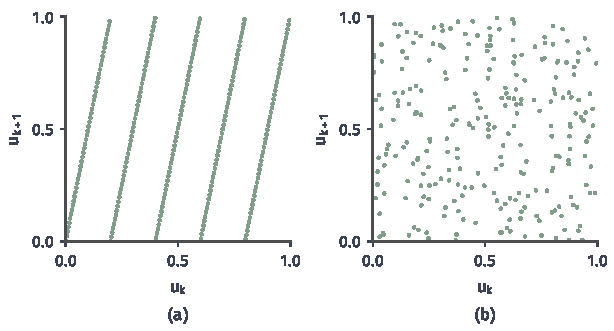
\includegraphics[width=104mm]{figures/07-probability/08-sampling-and-integration/matplotlib/sgen-lcg-pairs/figure.pdf}
  \caption{相邻伪随机数$(u_k,u_{k+1})$组成的点。(a)线性同余递推$s_{k+1}=(5s_k+1)\bmod256$，种子$s_0=7$，一个完整周期的$256$个点全部落在斜率为$5$的五条线段上；(b)NumPy的PCG64生成器，种子$7$，$256$对数。两者的单个$u_k$都在$[0,1)$上均匀分布，差别只在相邻数的联合分布上。}
  \label{fig:sgen-lcg-pairs}
\end{BookInlineFigure}

实用的生成器周期极长（例如$2^{128}$量级），并通过了大量针对相邻数、长程相关和高维分布的统计检验\scite{math-knuth1997seminumerical}。检验通过只说明没有发现所测试的那类偏差，并不证明序列与理想模型无法区分。本卷此后的推导都在理想模型下进行，把“伪随机数足够接近理想模型”当作一个外部假设。

\paragraph{种子与复现}
固定种子，同一程序就产生同一串数，整个计算可以逐位复现。这对查错和比较方法很有用：改动一处代码后用同一种子重跑，结果的变化只来自改动本身。本卷图中的模拟都注明了种子。

复现不等于验证。一个错误的生成方法在固定种子下同样给出可复现的错误结果；某个种子下直方图“看起来对”，换一个种子也可能仍然看起来对，因为错误可能只出现在很少被抽到的区域。生成方法是否正确，要靠式~\eqref{eq:sgen-correct-law}那样的证明，再加上第~\ref{sec:sgen-checks}节的检查；种子只负责让计算可以重来一遍。

\paragraph{有限精度}
浮点数格式也会改变理想模型。常见的双精度均匀数取值于$\{k2^{-53}:k=0,1,\dots,2^{53}-1\}$，可能取到$0$，取不到$1$。若后续要计算$\ln u$，取到$0$就会出错，所以要先确认生成器的取值范围，必要时改用$1-u$。格点还截断了尾部：由$-\ln(1-u)$生成的指数样本不会超过$53\ln2\approx36.7$。对指数分布，被截去的概率约为$\mathrm{e}^{-36.7}$，可以忽略；对尾部很重的分布或专门研究稀有事件的计算，这种截断就需要单独检查。
